\chapter{Analyse et solutions du problème}
\chaptermark{Analyse du P}

\section{Introduction et choix du langage}
Dans le cadre du module Systèmes Distribués, l'opportunité de  spécifier et concevoir  un générateur de tâches temps réel nous est proposé. Le langage d'implémentation étant libre, notre binome a opté pour Java. Ce choix est basé principalement par le fait qu'il s'agissait du langage le plus maitrisé. Cela nous a permis de concentrer nos efforts sur la mise en place des algorithmes et non sur des probèmes de langage.
 L'objectif est de définir un outil de simulation  d'ordonancement de tâche en temps réel.

\section{Modelisation du problème}
Le cahier des charges demandait une gestion de taches périodique et apériodiques. blah blah blah d'ordonancement
\section{Génération de tâches dans un fichier}
\sectionmark{Génération fichier}
La première partie du projet avait pour objectif d'obtenir un nombre n de taches périodiques et apériodiques pour de futurs traitements décrits dans la partie 2 : rajouter lien dym. \'A nouveau le choix du format d'un tel fichier nous était laissé. Nous avons choisis de générer un fichier xml (à nouveau pour des raisons  de simplicité) à la syntaxe suivante : 

\begin{itemize}
\item
Des balises \verb+<genTache.AbstractTache-array>+ encadrent la totalité du fichier.
\item
Une tâche périodique sera définie dans une balise  \verb+<genTache.TachePeriodique>+ 
\item
Une tâche apériodique sera définie dans une balise  \verb+<genTache.TacheAPeriodique>+ 
\item
Dans une tache tous ses attributs seront définis de la manière suivante \verb+<nom_attribut>valeur_attribut</nom_attribut>+
\end{itemize}

Voici un exemple d'un respectant le format décrit ci-dessus : 

\begin{lstlisting}
<genTache.AbstractTache-array>
  <genTache.TachePeriodique>
    <Pi>377</Pi>
    <ri>0</ri>
    <id>1</id>
    <Ci>1</Ci>
    <Di>1</Di>
  </genTache.TachePeriodique>
  <genTache.TachePeriodique>
    <Pi>162</Pi>
    <ri>0</ri>
    <id>2</id>
    <Ci>6</Ci>
    <Di>30</Di>
  </genTache.TachePeriodique>
  <genTache.TacheAperiodique>
    <ri>859</ri>
    <id>3</id>
    <Ci>26</Ci>
    <Di>71</Di>
  </genTache.TacheAperiodique>
</genTache.AbstractTache-array>
\end{lstlisting}
On remarque que les taches périodiques sont identifiées par : 
\begin{itemize}
\item
Pi : période d'activation.
\item
ri : date de réveil.
\item
id : L'id de la tâche.
\item
Ci : durée d'exécution maximale.
\item
Di  : délai critique
\end{itemize} 
Alors que les tâches apériodiques ont seulement : 
\begin{itemize}
\item
ri  : date de réveil
\item
id : L'id de la tâche.
\item
Ci : durée d'exécution maximale.
\item
Di : délai critique.
\end{itemize} 
\section{Algorithmes et structures mises en oeuvre}
\sectionmark{Algorithmes}
\subsection{Première Partie}
   \begin{figure}[htbp]
  \centering
  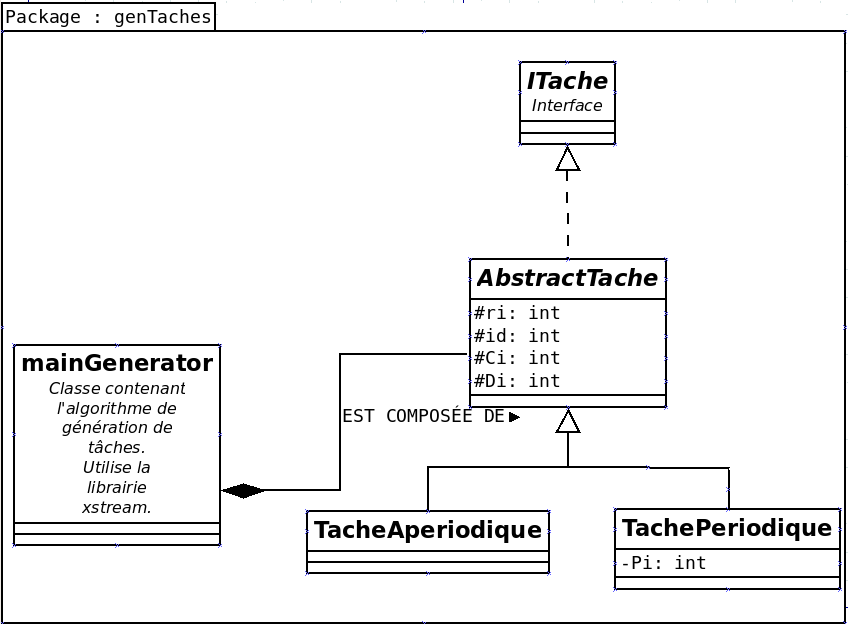
\includegraphics[scale=0.60]{img/packgen}
  \caption{Package générateur de tâches temps réel}
  \label{fig:gen}
\end{figure}

Calcul des tâches ap  
Le calcul des tâches ap est effectué selon la formule suivante : $ U_a =  \frac{\sum_{i=1}^m C_i}{ppcm(P_i)}$   ....  L'utilisateur entre la variable Uap  et le nombre de tache ap qu'il désire (m) les variables restantes 
charge des ap sur une hyperpériode 

\subsection{Deuxième partie}
La deuxième partie du projet, consistait à partir du fichier de tâches (cf Première Partie), de creer un simulateur proposant  deux types de fonctionnalités :
\begin{itemize}
\item
une analyse d'ordonnançabilité,
\item
un environnement de simulation.
\end{itemize}
Le premier sujet de reflexion était donc dans quelles structures de donnée stocker les tâches et par quels moyens. Le choix des ArrayList s'est fait naturellement grâce en premier plan à sa facilité de manipulation. Par ailleurs la fonctionnalité de la bibliothèque xtream permettant d'extraire le contenu d'un fichier xml dans une ArrayList en quelques lignes nous a d'emblée convaincu. Une fois cette première difficulté franchie une seconde de taille est apparue. Nous avons compris qu'il serait délicat de modifier directement les tâches dans les ArrayList. Notre idée initiale était de  modifier son Ci d'une  tâche après sont traitement dans l'algorithme. Ce qui dans le cas des tâches périodique par exemple, serait problématique. En effet par définition les taches périodiques  sont suseptible à être traitésà plusieurs reprise. Il faut donc garder leurs propiétés initiales intactes. Nous avons donc choisi d'organiser notre programmation en plusieurs classes pour bien séparer les opérations de manipulation des données d'une part, les opérations mettant en jeux les algorithmes d'ordonancement et enfin celles écrivant dans le fichier de sortie au format .ktr

   \begin{figure}[htbp]
  \centering
  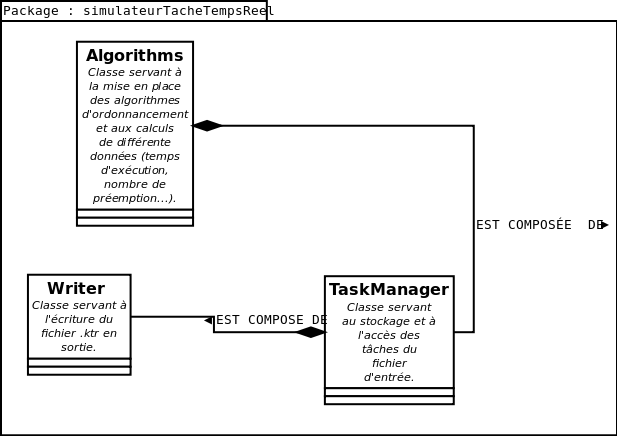
\includegraphics[scale=0.60]{img/packsstr}
  \caption{Package : Simulateur de systèmes temps réel}
  \label{fig:sstr}
\end{figure}
\clearpage
\section{Interface proposée}
Toutes l'interface de l'outil est en ligne de commande. L'absence d'IHM graphique est due au manque de temps et au peu d'intêret que cela représentait pour le problème étudié. De même l'outil ne prend en compte aucune option. Même si cet aspect aurait apporté un certain confort à l'utilisateur, nous avons opté pour la solution de lui demandé au fur et à mesur de l'execution du programme les diverses options et paramètres requis. Nous avons regretté ce choix lors de la phase des test (la répétitions sans cesse des divers option est fastidieuse). Cependant nous avons gagné un temps de conceptio non négligeable. 


